\documentclass[14pt,]{article}
\usepackage{lmodern}
\usepackage{amssymb,amsmath}
\usepackage{ifxetex,ifluatex}
\usepackage{fixltx2e} % provides \textsubscript
\ifnum 0\ifxetex 1\fi\ifluatex 1\fi=0 % if pdftex
  \usepackage[T1]{fontenc}
  \usepackage[utf8]{inputenc}
\else % if luatex or xelatex
  \ifxetex
    \usepackage{mathspec}
  \else
    \usepackage{fontspec}
  \fi
  \defaultfontfeatures{Ligatures=TeX,Scale=MatchLowercase}
    \setsansfont[]{GFS Neohellenic}
\fi
% use upquote if available, for straight quotes in verbatim environments
\IfFileExists{upquote.sty}{\usepackage{upquote}}{}
% use microtype if available
\IfFileExists{microtype.sty}{%
\usepackage{microtype}
\UseMicrotypeSet[protrusion]{basicmath} % disable protrusion for tt fonts
}{}
\usepackage[margin=1in]{geometry}
\usepackage{hyperref}
\hypersetup{unicode=true,
            pdftitle={Overview and illustration of methods to investigate effect modification across a continuous covariate},
            pdfauthor={Michail Belias},
            pdfborder={0 0 0},
            breaklinks=true}
\urlstyle{same}  % don't use monospace font for urls
\usepackage{graphicx,grffile}
\makeatletter
\def\maxwidth{\ifdim\Gin@nat@width>\linewidth\linewidth\else\Gin@nat@width\fi}
\def\maxheight{\ifdim\Gin@nat@height>\textheight\textheight\else\Gin@nat@height\fi}
\makeatother
% Scale images if necessary, so that they will not overflow the page
% margins by default, and it is still possible to overwrite the defaults
% using explicit options in \includegraphics[width, height, ...]{}
\setkeys{Gin}{width=\maxwidth,height=\maxheight,keepaspectratio}
\IfFileExists{parskip.sty}{%
\usepackage{parskip}
}{% else
\setlength{\parindent}{0pt}
\setlength{\parskip}{6pt plus 2pt minus 1pt}
}
\setlength{\emergencystretch}{3em}  % prevent overfull lines
\providecommand{\tightlist}{%
  \setlength{\itemsep}{0pt}\setlength{\parskip}{0pt}}
\setcounter{secnumdepth}{0}
% Redefines (sub)paragraphs to behave more like sections
\ifx\paragraph\undefined\else
\let\oldparagraph\paragraph
\renewcommand{\paragraph}[1]{\oldparagraph{#1}\mbox{}}
\fi
\ifx\subparagraph\undefined\else
\let\oldsubparagraph\subparagraph
\renewcommand{\subparagraph}[1]{\oldsubparagraph{#1}\mbox{}}
\fi

%%% Use protect on footnotes to avoid problems with footnotes in titles
\let\rmarkdownfootnote\footnote%
\def\footnote{\protect\rmarkdownfootnote}

%%% Change title format to be more compact
\usepackage{titling}

% Create subtitle command for use in maketitle
\newcommand{\subtitle}[1]{
  \posttitle{
    \begin{center}\large#1\end{center}
    }
}

\setlength{\droptitle}{-2em}

  \title{Overview and illustration of methods to investigate effect modification
across a continuous covariate}
    \pretitle{\vspace{\droptitle}\centering\huge}
  \posttitle{\par}
    \author{Michail Belias}
    \preauthor{\centering\large\emph}
  \postauthor{\par}
      \predate{\centering\large\emph}
  \postdate{\par}
    \date{10 oktober, 2018}

\usepackage{booktabs}
\usepackage{longtable}
\usepackage{array}
\usepackage{multirow}
\usepackage[table]{xcolor}
\usepackage{wrapfig}
\usepackage{float}
\usepackage{colortbl}
\usepackage{pdflscape}
\usepackage{tabu}
\usepackage{threeparttable}
\usepackage{threeparttablex}
\usepackage[normalem]{ulem}
\usepackage{makecell}

\usepackage{bbm}
\usepackage{booktabs}
\usepackage{longtable}
\usepackage{array}
\usepackage{dsfont}
\usepackage{multirow}
\usepackage[table]{xcolor}
\usepackage{wrapfig}
\usepackage{float}
\usepackage{colortbl}
\usepackage{pdflscape}
\usepackage{tabu}
\usepackage{threeparttable}
\usepackage{threeparttablex}
\usepackage[normalem]{ulem}
\usepackage{makecell}
\newcommand{\blandscape}{\begin{landscape}}
\newcommand{\elandscape}{\end{landscape}}

\begin{document}
\maketitle

\section{Abstract (116 out of 200
words)}\label{abstract-116-out-of-200-words}

\subsection{Objective}\label{objective}

To overview and illustrate a variety of tree-based and regression-based
approaches to detect and model effect-modification in meta-analysis(MA)
of individual participant data(IPD), such as: covariate-centred IPD-MA,
mixed effects fractional polynomials, splines, meta-stepp and
glmm-trees.

\subsection{Study Design and Setting}\label{study-design-and-setting}

We applied the aforementioned approaches into two empirical data-sets.
The first is investigating the effect of somatostatin treatment versus
placebo in liver reduction percentage, on participants with polycystic
liver disease. The second investigates the effect of antibiotics in
fever/ear-pain reduction, on children with acute otitis media(AOM).

\subsection{Results}\label{results}

Non-linear association was detected in AOM IPD-MA.

\subsection{Conclusion}\label{conclusion}

We conclude that subgroup detection in IPD-MA requires knowing the
underlying assumptions and careful modelling. Effect modification may be
distorted by a non-linear association if left unadjusted.

\newpage

\subparagraph{}\label{section}

\section{1. Introduction}\label{introduction}

\par      

Individual participant data meta-analysis (IPD-MA) is a type of
systematic review, where data gathered from multiple studies are
combined and analysed centrally. The capability to standardise subgroup
definitions and outcomes across studies, the increased power to
investigate other than linear associations, the increased validity and
reliability of the subgroups and the flexibility to search for subgroups
based on combinations of patient and/or disease characteristics are some
of the benefits of using IPD of multiple trials rather than traditional
(aggregate) meta-analysis. A vivid field of research towards
personalised healthcare is the investigation of effect modification. For
this task, IPD-MA is considered a gold standard as single trials rarely
have sufficient power to identify relevant effect modification.
\par      Effect modification is known to be present in both categorical
and/or continuous covariates. For example, differences in the treatment
effect may be present between smokers and non-smokers. In this case,
subgroups are already defined and therefore, only confirmatory
hypothesis testing may be conducted. The investigation of subgroup
effects is performed using statistical tools, such as generalised linear
models combined with meta-analytical tools, or generalised linear
mixed-effects models with interaction terms included. Subsequently, the
estimated coefficients are checked for statistical significance. On the
other hand, effect modification across a continuous covariate is more
challenging, as the subgroups are non-existent or not be a-priori known.
A common technique is to categorise the continuous covariate. Thereto,
subgroups are generated using prior knowledge driven from literature.
Nevertheless, categorisation has been criticised for misspecification,
loss of information and power, inflation of the type I error rate when
adjusting for confounding and biased results {[}1--5{]}. Another common
practice is to assume linearity over the link function, a method that
may also lead to deterioration of power, misspecification and even
spurious results {[}6{]}. Therefore, besides confirming a variable if is
an effect modifier, we may have to the explore the functional form of
the outcome-effect modifier association. Various approaches to account
for non-linear associations have been developed, such as: fractional
polynomials {[}7{]} and splines. \par      Regression based approaches
such as: linear models, piecewise polynomials or fractional polynomials
may be performed either in one or two stages. In two-stage approach,
each trial is first modelled separately, using an appropriate
statistical model of choice. Subsequently, we pool either the extracted
estimates or the fitted functions across trials using standard
meta-analytical tools. In contrast, in one-stage IPD-MA all IPD from
every trial are analysed simultaneously whilst accounting for the
clustering of participants within studies. Hereto, researchers may model
interactions between treatment and patient-level covariates. Recent
recommendations, suggest mean-centring the potential effect modifiers
per trial in order to account for potential ecological bias due to
unadjusted confounding. Within trials clustering can be accounted using
either fixed effect\textbf{s} (stratified intercept/slope), fixed effect
(common intercept/slope) or random effects (intercept and/slopes driven
from a common Normal distribution) {[}9{]}. Finally, state-of-the-art
plot and tree-based methods have been developed for exploring and
confirming effect modification. Generalised linear mixed-effects model
trees (glmertree) introduced by Fokkema et al.{[}10{]} can handle
non-linear associations, whilst accounting for within studies clustering
of the participants. Meta-stepp is a plot based moving average (sliding
window) method that approximates non-linear effects from clustered data
{[}11{]}. Finally, although, providing the whole information of the
outcome-continuous effect modifier association is more informative
clinical decisions are based in cut-points in which the treatment effect
is altered. These cut-points may be altered if the assumptions are
altered or if the outcome-effect modifier functional form is
mis-specified. \par
 It is often unclear when each method should be preferred. Also, it is
unclear if the treatment effect function {[}12{]} or interaction term
analysis {[}13{]} is most appropriate and in randomised clinical trials
(RCT) meta-analysis framework. We aim to describe and illustrate the
aforementioned methods. For that task, we will use both regression-based
approaches such as meta-stepp, centred one-stage IPD-MA, mixed effects
fractional polynomials and splines, and tree-based approaches such as
generalised linear mixed-effects model trees.

\section{2. Data}\label{data}

We use 2 empirical IPD-sets. The first data-set {[}14{]} was
investigating the effect of antibiotics in acute otitis media on
children aged from 0 to 12 years old. Rovers et al. collected IPD from 6
randomised clinical trials with a total of 1643 children, aged from 0-12
years old. The primary outcome was fever and/or ear-pain after 3-7 days
(yes/no). Rovers et al. concluded that antibiotics were more beneficial
in younger children (less than 2 years old) with bilateral acute otitis
media. Bilateral acute otitis media (yes/no), age, otorrhea were also
investigated separately for potential effect modification and only
bilateral acute otitis media showed a significant result.

The second data-set {[}15{]} was investigating the effect of
somatostatin in the liver volume reduction. Gevers et al. collected IPD
from 3 randomised placebo-controlled trials with a total of 107
participants. The outcome was continuous (liver volume reduction) and
age, sex, baseline liver volume, and diagnosis of autosomal dominant
polycystic liver or kidney disease has been investigated for effect
modification. Gevers et al. concluded that therapy using somatostatin
was more beneficial for young female patients. One of the included
trials {[}Caroli et al.{]} had a cross-over design, therefore
participants were in both treatment groups (control and treated) in
different time periods. We matched the participants per age and gender
and picked half on the treated and half on the control group. Therefore,
some differences between our results and those reported in the original
article may occur.

\section{3. Methods}\label{methods}

\subsection{3.1 Notation}\label{notation}

We are denoting the studies as j = 1,2,\ldots{},J, individuals as
i=1,2\ldots{},I, the per trial mean of age as \(\bar{Age_j}\), cut-point
as \(\kappa\)

\subsection{3.2. Recursive-partitioning (tree-based)
methods}\label{recursive-partitioning-tree-based-methods}

\subsubsection{3.2.1 Generalised Linear Mixed Model Trees (glmm or glmer
trees)}\label{generalised-linear-mixed-model-trees-glmm-or-glmer-trees}

Generalised linear mixed model trees approach is a state-of-the-art
technique, proposed by Fokkema et al {[}10{]} for the detection of
treatment-effect modifier interaction. A model-based recursive
partitioning {[}16,17{]} algorithm is applied, while also considering
the clustered structure of datasets.

The GLMM tree algorithm:

\begin{enumerate}
\def\labelenumi{(\arabic{enumi})}
\tightlist
\item
  fit the parametric model to the dataset,
\item
  statistically test for parameter instability with respect to each of a
  set of partitioning variables,
\item
  if there is some overall parameter instability, split the dataset with
  respect to the variable associated with the highest instability,
\item
  repeat the procedure in each of the resulting subgroups.
\end{enumerate}

\subparagraph{}\label{section-1}

\newpage

\subsection{3.3 Regression based
approaches}\label{regression-based-approaches}

We identify 2 assumptions that a researcher may have. The first is over
the functional form the the association of the outcome with the
continuous covariate have and the second one over the cut-points known
also as cut-offs or knots, where the effect is modified. In this
framework, we consider that given the assumptions made we may choose the
appropriate analysis to perform.

\begin{figure}
\centering
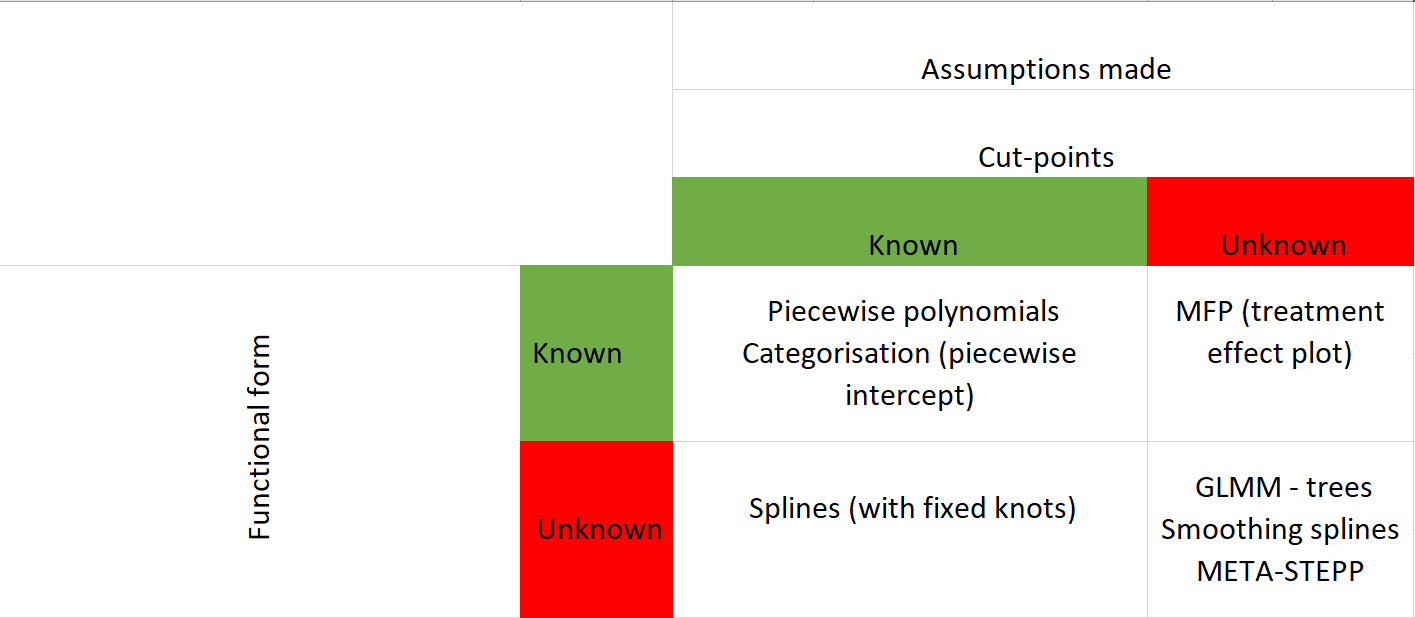
\includegraphics{Figs/Assumption.png}
\caption{Table 1}
\end{figure}

\subsubsection{3.3.1. Two-stage approaches}\label{two-stage-approaches}

In two-stage approaches a statistical model of choice is directly fitted
per trial. The statistical model per trial j is as follows:

\(g(Y_{ij}) = f_1(Age) + f_2(Age) \times Treatment\)

Subsequently, we can either pool the coefficients or the fitted
functions using typical meta-analytical tools.

\paragraph{3.3.1.1 First stage: Per-trial
modeling}\label{first-stage-per-trial-modeling}

\emph{Known functional form and known cut-points}

The functions \(f_1, f_2\) are providing the functional shape of
outcome-effect modifier for the treated and the control respectively.
Depending on the apriori knowledge of the outcome- effect modifier
functional form and the cut-points where the effect is altered we may
fit.

\begin{itemize}
\tightlist
\item
  Piecewise-polynomials with m cut-points (knots)
  \[f_1 = \sum_{\kappa =1}^{\kappa= m}f_{1\kappa}(X_{x_{k-1} \leq X < x_{k-1}} ), f_2 =  \sum_{\kappa =1}^{\kappa= m}f_{2\kappa}(X_{x_{k-1} \leq X < x_{k-1}} )\]

  \begin{itemize}
  \tightlist
  \item
    Piecewise intercept: within each interval \(\omega\) both f1,f2 have
    the form of \(\beta_{\omega}\) (equivalent to Dichotomisation for
    k=2 and categorisation k\textgreater{}2)
  \item
    Piece-linear: within each interval \(\omega\) both f1,f2 have the
    form of \(\beta_{\omega} \times X\)
  \item
    Piece-linear: within each interval \(\omega\) both f1,f2 have the
    form of \(\beta_{\omega} \times X^2\)
  \end{itemize}
\item
  Global-polynomials:
  \[f_1 =  \sum_{p=1}^{p=m} \beta_{1p} \times X^p , f_2 = \sum_{p=1}^{p=m} \beta_{2p} \times X^p\]

  \begin{itemize}
  \tightlist
  \item
    linear:
    \(f_1 = \beta_{10} + \beta_{11} \times X , f_2 = \beta_{20} + \beta_{21} \times X\)
  \item
    Quadratic:
    \(f_1 = \beta_{10} + \beta_{11} \times X + \beta_{12} \times X^2 , f_2 = \beta_{20} + \beta_{21} \times X + \beta_{22} \times X^2\)
  \end{itemize}
\end{itemize}

\paragraph{Fractional polynomials}\label{fractional-polynomials}

Fractional polynomials {[}18{]} are an extension of typical polynomials,
that also include negative powers. The fractional polynomials model the
effect of an covariate X as
\(f(x;\beta) = \sum_{k=1}^{k=m} \beta_{k} \times X^{p_{k}}\), where m is
the degree of the fractional polynomial and the \(p_k \in S :\)
\{-2,-1,-0.5, 0=(log),0.5,1,2\}. An algorithm (FSP) has been proposed
{[}19{]} to explore the best fitting fractional polynomial, where all
fractional polynomials of common degree are tested using the deviance
difference criterion, while the best fitting fractional polynomials of
different degree are compared using a \(\chi^2\) test. When multiple
data-sets are present Sauerbrei and Royston {[}7{]}, have proposed 3
methods to produce a general functional form.

\begin{itemize}
\tightlist
\item
  Overall FP, where the FSP is applied in the pooled data , to find the
  best FP (stratified by data-set).
\item
  Study-wise FP2, the best FP2 is selected for each study
\item
  Study wise selected FP, where the best fitting FP is extracted per
  study
\end{itemize}

\paragraph{3.3.1.2 Second-stage}\label{second-stage}

As a second-stage in the two-stage IPD-MA, we either pool the estimates
or the fitted functions extracted from the first stage.

\subsubsection{3.3.2. One-stage approach}\label{one-stage-approach}

\paragraph{3.3.2.1 Centred One-stage
IPD-MA}\label{centred-one-stage-ipd-ma}

We follow recent recommendations {[}21{]} and centre per trial the
effect modifier. This way we separate the within and across trial
information. Recent recommendations propose to mean centre the
continuous covariate in order to separate within and across trial
heterogeneity {[}21{]}. Assuming the \(X_{ij} = Age_{ij} - \bar Age_j\)

\(g(Y_{ij}) = \beta_{0j} + \beta_{Tj} \times Treatment + \beta_{Aj} \times( Age_{ij} - \bar{Age_{j}}) + \beta_{xj} \times Treatment \times ( Age_{ij} - \bar{Age_{j}}))\)

\(\beta_{0j} \sim N(\beta_{0}, \tau_{0}^2)\)

\(\beta_{Tj} \sim N(\beta_{T}, \tau_{T}^2)\)

\(\beta_{Aj} \sim N(\beta_{A}, \tau_{A}^2)\)

\(\beta_{xj} \sim N(\beta_{x}, \tau_{x}^2)\)

\subsection{Mixed effect fractional
polynomials}\label{mixed-effect-fractional-polynomials}

We follow recent recommendations {[}21{]} and centre per trial the
effect modifier. This way we separate the within and across trial
information.

\(g(Y_{ij}) = \beta_{0j} + \beta_{Tj} \times Treatment + \beta_{Aj} \times fp( Age - \bar{Age}) + \beta_{xj} \times Treatment \times fp( Age - \bar{Age}))\)

mixed

\(\beta_{0j} \sim N(\beta_{0}, \tau_{0}^2)\)

\(\beta_{Tj} \sim N(\beta_{T}, \tau_{T}^2)\)

\(\beta_{Aj} \sim N(\beta_{A}, \tau_{A}^2)\)

\(\beta_{xj} \sim N(\beta_{x}, \tau_{x}^2)\)

\newpage

\subparagraph{}\label{section-2}

\newpage

\subparagraph{}\label{section-3}

\section*{References}\label{references}
\addcontentsline{toc}{section}{References}

\hypertarget{refs}{}
\hypertarget{ref-Royston_2005}{}
{[}1{]} Royston P, Altman DG, Sauerbrei W. Dichotomizing continuous
predictors in multiple regression: A bad idea. Statistics in Medicine
2005;25:127--41.
doi:\href{https://doi.org/10.1002/sim.2331}{10.1002/sim.2331}.

\hypertarget{ref-Altman_2006}{}
{[}2{]} Altman DG. The cost of dichotomising continuous variables. BMJ
2006;332:1080--0.
doi:\href{https://doi.org/10.1136/bmj.332.7549.1080}{10.1136/bmj.332.7549.1080}.

\hypertarget{ref-Austin_2004}{}
{[}3{]} Austin PC, Brunner LJ. Inflation of the type i error rate when a
continuous confounding variable is categorized in logistic regression
analyses. Statistics in Medicine 2004;23:1159--78.
doi:\href{https://doi.org/10.1002/sim.1687}{10.1002/sim.1687}.

\hypertarget{ref-Maxwell_1993}{}
{[}4{]} Maxwell SE, Delaney HD. Bivariate median splits and spurious
statistical significance. Psychological Bulletin 1993;113:181--90.
doi:\href{https://doi.org/10.1037/0033-2909.113.1.181}{10.1037/0033-2909.113.1.181}.

\hypertarget{ref-Weinberg_1995}{}
{[}5{]} Weinberg C. How bad is categorization? Epidemiology
1995;6:345--6.
doi:\href{https://doi.org/10.1097/00001648-199507000-00002}{10.1097/00001648-199507000-00002}.

\hypertarget{ref-J_rgensen_2016}{}
{[}6{]} Jørgensen TSH, Osler M, Ängquist LH, Zimmermann E, Christensen
GT, Sørensen TI. The u-shaped association of body mass index with
mortality: Influence of the traits height, intelligence, and education.
Obesity 2016;24:2240--7.
doi:\href{https://doi.org/10.1002/oby.21615}{10.1002/oby.21615}.

\hypertarget{ref-Sauerbrei_2011}{}
{[}7{]} Sauerbrei W, Royston P. A new strategy for meta-analysis of
continuous covariates in observational studies. Statistics in Medicine
2011;30:3341--60.
doi:\href{https://doi.org/10.1002/sim.4333}{10.1002/sim.4333}.

\hypertarget{ref-royston_interaction_2013}{}
{[}8{]} Royston P, Sauerbrei W. Interaction of treatment with a
continuous variable: Simulation study of significance level for several
methods of analysis. Statistics in Medicine 2013;32:3788--803.
doi:\href{https://doi.org/10.1002/sim.5813}{10.1002/sim.5813}.

\hypertarget{ref-Legha_2018}{}
{[}9{]} Legha A, Riley RD, Ensor J, Snell KI, Morris TP, Burke DL.
Individual participant data meta-analysis of continuous outcomes: A
comparison of approaches for specifying and estimating one-stage models.
Statistics in Medicine n.d.;0.
doi:\href{https://doi.org/10.1002/sim.7930}{10.1002/sim.7930}.

\hypertarget{ref-Fokkema_2017}{}
{[}10{]} Fokkema M, Smits N, Zeileis A, Hothorn T, Kelderman H.
Detecting treatment-subgroup interactions in clustered data with
generalized linear mixed-effects model trees. Behavior Research Methods
2017.
doi:\href{https://doi.org/10.3758/s13428-017-0971-x}{10.3758/s13428-017-0971-x}.

\hypertarget{ref-Wang_2016}{}
{[}11{]} Wang XV, Cole B, Bonetti M, Gelber RD. Meta-STEPP:
Subpopulation treatment effect pattern plot for individual patient data
meta-analysis. Statistics in Medicine 2016;35:3704--16.
doi:\href{https://doi.org/10.1002/sim.6958}{10.1002/sim.6958}.

\hypertarget{ref-Royston_2008}{}
{[}12{]} Royston P, Sauerbrei W. Interactions between treatment and
continuous covariates: A step toward individualizing therapy. Journal of
Clinical Oncology 2008;26:1397--9.
doi:\href{https://doi.org/10.1200/jco.2007.14.8981}{10.1200/jco.2007.14.8981}.

\hypertarget{ref-Sun_2010}{}
{[}13{]} Sun X, Briel M, Walter SD, Guyatt GH. Is a subgroup effect
believable? Updating criteria to evaluate the credibility of subgroup
analyses. BMJ 2010;340:c117--7.
doi:\href{https://doi.org/10.1136/bmj.c117}{10.1136/bmj.c117}.

\hypertarget{ref-Rovers_2006}{}
{[}14{]} Rovers MM, Glasziou P, Appelman CL, Burke P, McCormick DP,
Damoiseaux RA, et al. Antibiotics for acute otitis media: A
meta-analysis with individual patient data. The Lancet
2006;368:1429--35.
doi:\href{https://doi.org/10.1016/s0140-6736(06)69606-2}{10.1016/s0140-6736(06)69606-2}.

\hypertarget{ref-Gevers_2013}{}
{[}15{]} Gevers TJ, Inthout J, Caroli A, Ruggenenti P, Hogan MC, Torres
VE, et al. Young women with polycystic liver disease respond best to
somatostatin analogues: A pooled analysis of individual patient data.
Gastroenterology 2013;145:357--365.e2.
doi:\href{https://doi.org/10.1053/j.gastro.2013.04.055}{10.1053/j.gastro.2013.04.055}.

\hypertarget{ref-Zeileis_2008}{}
{[}16{]} Zeileis A, Hothorn T, Hornik K. Model-based recursive
partitioning. Journal of Computational and Graphical Statistics
2008;17:492--514.
doi:\href{https://doi.org/10.1198/106186008x319331}{10.1198/106186008x319331}.

\hypertarget{ref-Su_2009}{}
{[}17{]} Su X, Tsai C-L, Wang H, Nickerson DM, Li B. Subgroup analysis
via recursive partitioning. SSRN Electronic Journal 2009.
doi:\href{https://doi.org/10.2139/ssrn.1341380}{10.2139/ssrn.1341380}.

\hypertarget{ref-Royston_1994}{}
{[}18{]} Royston P, Altman DG. Regression using fractional polynomials
of continuous covariates: Parsimonious parametric modelling. Applied
Statistics 1994;43:429.
doi:\href{https://doi.org/10.2307/2986270}{10.2307/2986270}.

\hypertarget{ref-Ambler_2001}{}
{[}19{]} Ambler G, Royston P. Fractional polynomial model selection
procedures: Investigation of type i error rate. Journal of Statistical
Computation and Simulation 2001;69:89--108.
doi:\href{https://doi.org/10.1080/00949650108812083}{10.1080/00949650108812083}.

\hypertarget{ref-Sauerbrei_1999}{}
{[}20{]} Sauerbrei W, Royston P. Building multivariable prognostic and
diagnostic models: Transformation of the predictors by using fractional
polynomials. Journal of the Royal Statistical Society: Series A
(Statistics in Society) 1999;162:71--94.
doi:\href{https://doi.org/10.1111/1467-985x.00122}{10.1111/1467-985x.00122}.

\hypertarget{ref-Hua_2016}{}
{[}21{]} Hua H, Burke DL, Crowther MJ, Ensor J, Smith CT, Riley RD.
One-stage individual participant data meta-analysis models: Estimation
of treatment-covariate interactions must avoid ecological bias by
separating out within-trial and across-trial information. Statistics in
Medicine 2016;36:772--89.
doi:\href{https://doi.org/10.1002/sim.7171}{10.1002/sim.7171}.


\end{document}
